\vspace{-.4em}
\section{Experiments}\label{sec:exp}
\vspace{-.4em}

\myparagraph{Dataset.} 
We evaluate the proposed methods on the MultiWOZ 2.0 dataset \citep{multiwoz2018}, which is a representative ToD benchmark.
MultiWOZ 2.0 is a large-scale multi-domain dialogue corpus 
% consisting of conversations between a tourist/user and a clerk/system at an information center of a tourist city.
with seven domains:  attraction, hospital, police, hotel, restaurant, taxi, and train. Each dialogue therein covers between one to three domains.
This dataset has $8438$ dialogues in the training set and $1000$ dialogues in the validation and test set respectively.

\myparagraph{Evaluation Metrics.} 
Our proposed method is evaluated on the E2E dialogue-modeling task of the MultiWOZ 2.0 dataset.
Following the standard setup \citep[\eg,][]{multiwoz2018,sfnrl2019}, we use four automatic evaluations metrics:
1) \textbf{Inform} rate: the fraction of the dialogues where the system has provided an appropriate entity;
2) \textbf{Success} rate: the fraction of the dialogues where the system answered all the requested information;
3) \textbf{BLEU} score \citep{bleu2002}: measures the fluency of the generated responses;
4) \textbf{Combined Score} \citep{sfnrl2019}: an overall quality measure defined as $\mathrm{Combined~Score} =: (\mathrm{Inform} + \mathrm{Success}) \times 0.5 + \mathrm{BLEU}$.
% All our provided results are the average over five random seeds.
Details on prepossessing and implementation are in Appendix~\ref{sec:algo_box} and~\ref{sec:impl_details}.


\begin{savenotes}
\begin{table}[tb] 
\vspace{-2mm}
\captionsetup{font=small}
\caption{
\footnotesize{Results of the E2E response generation task on the MultiWOZ 2.0 dataset.
The best result on each metric is bold.
The results of UBAR are from the reproduction by \citet{gptcritic2022}.
The results of CASPI are from our reproduction.
All our provided results are the average over five random seeds.
Other results are from the original paper.
``GS" denotes the Gumbel-softmax trick.
$(\cdot)^{1}$ denotes the power function with power $1$.}
} 
\label{table:main} 
\vspace{-.7em}
\centering 
% \def\arraystretch{1.2}
% \setlength\tabcolsep{15pt}
\resizebox{.70\textwidth}{!}{
\begin{tabular}{@{}lcccc@{}}
\toprule
Algorithms                                           & Inform & Success & BLEU  & Combined Score \\ \midrule
SFN + RL    \citep{sfnrl2019}                                           & 73.80  & 53.60   & 16.90 & 83.10          \\
DAMD       \citep{damd2020}                                          & 76.40  & 64.35   & 17.96 & 88.34          \\
SimpleTOD \citep{simpletod2020} & 84.40  & 70.10   & 15.01 & 92.26          \\
MinTL     \citep{mintl2020}                                           & 84.88  & 74.91   & 17.89 & 97.78          \\
SOLOIST  \citep{soloist2021}                                            & 85.50  & 72.90   & 16.54 & 95.74          \\
UBAR \citep{ubar2021}                                                & 87.47  & 74.43   & 17.61 & 98.56          \\
GPT-Critic  \citep{gptcritic2022}                                         & 90.07  & 76.63   & 17.83 & 101.13         \\
CASPI\footnote{
The CASPI paper reports the median score over random seeds, instead of the more commonly used mean score.
We run the official CASPI codebase (\href{https://github.com/salesforce/CASPI}{https://github.com/salesforce/CASPI}) and report the mean scores.
}  \citep{caspi2021}                                              & 91.37  & 82.80   & 17.70 & 104.78         \\ 
\midrule
\texttt{RewardNet}, $N=3$, $\Phi=(\cdot)^{1}$ & 92.77 & 84.28 & 17.74 & 106.27 \\
\texttt{RewardMLE}, $N=5$, $\Phi=\exp(\cdot)$ & 91.49 & 83.38 & \textbf{18.97} & 106.40 \\
\texttt{RewardNet} + GS, $N=3$, $\Phi=(\cdot)^{1}$ & 92.63 & \textbf{84.32} & 18.35 & \textbf{106.83} \\
\texttt{RewardMLE} + GS, $N=5$, $\Phi=\exp(\cdot)$ & \textbf{93.09} & 83.90 & 18.04 & 106.54 \\
\bottomrule
\end{tabular}
}
\vspace{-1.5em}
\end{table}
\end{savenotes}

\vspace{-.4em}
\subsection{Main Results} \label{sec:exp_main} 
\vspace{-.4em}



\myparagraph{Main evaluation.} 
Table~\ref{table:main} compares the performance of our methods with several classical and recent approaches in the E2E response-generation task.
% outperforms baselines: good inform and success and good bleu score
As shown in Table~\ref{table:main}, our proposed methods not only improve the dialogue-task completion, measured by the Inform rate and the Success rate; but also generate fluent responses, reflected by the competitive BLEU scores.
% compare with CASPI (special case), 
Recall that CASPI is a special case of the \texttt{RewardNet} loss (Eq.~\eqref{eq:listnet}) when we use escort transform ($\Phi = (\cdot)^{1}$, the identity function) with pairwise preference ($N=2$).
%our proposed method when using the pairwise version of the ListNet loss and when the probabilistic transform in Eq.~\eqref{eq:listnet} is the escort transform with power one.
% using listwise ranking improve score (w. simple why?)
When we use three dialogue trajectories ($N=3$) to construct the \texttt{RewardNet} loss and retain the same escort transform, the overall performance generally improves over CASPI.
As discussed in \Secref{sec:main_rew_obj}, our \rewardnet loss generalizes the pairwise-preference learning by taking more information on each update of the reward model and thus could learn a better reward function.
Appendix~\ref{sec:detailed_comp_caspi} further compares our methods with CASPI.

% using listmle improves performances since it is more robust to the error in scores
The performance is further gently improved by changing the \rewardnet loss (Eq.~\eqref{eq:listnet}) to the \rewardmle loss (Eq.~\eqref{eq:listmle}), with the softmax transform ($\Phi = \exp(\cdot)$) and $N=5$ dialogue trajectories.
This again demonstrates the benefit of our proposal of using multiple trajectories to learn the reward model. \Secref{sec:exp_abla} conducts ablation studies on the number of trajectories and choice of $\Phi$.
% This gain may come from the relative robustness of the RewardMLE loss to small errors in the scoring process since the RewardMLE loss only uses the ranking of the provided scores, but not the numerical score values as in the RewardNet loss.

% Adding GS to both models further improve scores: directly optimize the learned reward func. is effective
So far, we follow the prior work to not utilize policy gradient to train the response-generation model, \ie, $\alpha=0$ in Eq.~\eqref{eq:loss_gen}.
Extra performance gain can be obtained by adding the policy-gradient updates via the Gumbel-softmax trick (GS) discussed in \Secref{sec:main_gs}.
Indeed, GS improves both the plain \rewardnet and \rewardmle models.
This shows the efficacy of directly optimizing the response-generation model \wrt~the learned reward function.
Further discussion is provided in \Secref{sec:exp_abla}.
% \yy{people may have questions that when we add gs, the performance boosted but rewardnet is better than rewardmle, contradictory with previous observation}

Appendix~\ref{sec:exp_galaxy} provides the experimental results when applying our method onto the recent  GALAXY backbone \citep{he2022galaxy}.
Appendix~\ref{sec:exp_multiwoz21} discusses the results on the MultiWOZ 2.1 dataset.

\myparagraph{Low-resource experiment.}
We evaluate our method on the low-data regime by following the testing strategy in \citet{mintl2020}.
Specifically, we use $5\%$, $10\%$, and $20\%$ of the training data to train our basic \rewardnet and \rewardmle models in Table~\ref{table:main}, without the GS component. 
We compare them with the baseline scores in \citet{mintl2020}.
Table~\ref{table:low_resource} reports the results.
It is clear that our models outperform the baselines, MinTL and DAMD, showing the efficacy of our method.
Compared with Table~\ref{table:main}, our models trained with $20\%$ of the data perform competitively with the baseline methods trained on the full training set.

\begin{table}[tb] 
\vspace{-2mm}
\captionsetup{font=small}
\caption{
\footnotesize{Results on the simulated low-resource settings, where $5\%$, $10\%$, and $20\%$ of the training data is used to train the models.
The best result on each metric under each setting is bold.
``Comb." is the Combined Score.
All our provided results are the average over five random seeds.
Baseline results are from \citet{mintl2020}.}
} 
\label{table:low_resource} 
\vspace{-.7em}
\centering 
% \def\arraystretch{1.2}
\resizebox{1.\textwidth}{!}{
\begin{tabular}{@{}ccccccccccccc@{}}
\toprule
\multirow{2}{*}{Model}     & \multicolumn{4}{c}{$5\%$}                              & \multicolumn{4}{c}{$10\%$}                            & \multicolumn{4}{c}{$20\%$}       \\
                           & Inform & Success & BLEU  & Comb.                      & Inform & Success & BLEU  & Comb.                      & Inform & Success & BLEU  & Comb. \\ \midrule
\multicolumn{1}{c|}{DAMD}  & 56.60  & 24.50   & 10.60 & \multicolumn{1}{c|}{51.15} & 62.00  & 39.40   & 14.50 & \multicolumn{1}{c|}{65.20}  & 68.30  & 42.90   & 11.80 & 67.40 \\
\multicolumn{1}{c|}{MinTL} & 75.48  & 60.96   & 13.98 & \multicolumn{1}{c|}{82.20}  & 78.08  & 66.87   & \textbf{15.46} & \multicolumn{1}{c|}{87.94} & 82.48  & 68.57   & 13.00 & 88.53 \\
\multicolumn{1}{c|}{\rewardnet:3} & 81.22  & 67.37   & 12.82 & \multicolumn{1}{c|}{87.11}  &   \textbf{92.39} & \textbf{78.98}   & 13.36 & \multicolumn{1}{c|}{\textbf{99.05}} & 89.83  &  \textbf{79.30}  & 15.18 & 99.75 \\
\multicolumn{1}{c|}{\rewardmle:5} & \textbf{82.90}  & \textbf{69.61}   & \textbf{14.26} & \multicolumn{1}{c|}{\textbf{90.51}}  & 89.67   &  77.48  & 14.80 & \multicolumn{1}{c|}{98.38} & \textbf{90.15}  &  78.70  & \textbf{15.81} & \textbf{100.24} \\
\bottomrule
\end{tabular}
}
\vspace{-1.0em}
\end{table}

\vspace{-.6em}
\subsection{Ablation Study} \label{sec:exp_abla}
\vspace{-.4em}
The ablation study considers the following four research questions to better understand our methods.

\textbf{(a):}~\textit{What if we learn the reward function via a different number of trajectories?}
In Fig.~\ref{fig:listnet_p1_num_traj} and \ref{fig:listmle_smax_num_traj}, we vary the number of trajectories used for the reward-learning losses in Table~\ref{table:main}.
To avoid unwanted interference, we use the basic version of models without the GS component.
The case of using two trajectories reduces to the pairwise-preference loss discussed in \Secref{sec:background}.

As shown in Fig.~\ref{fig:listnet_p1_num_traj} and \ref{fig:listmle_smax_num_traj}, our generalized approach of using multiple trajectories to learn the reward function provides the flexibility to outperform the classical pairwise-preference learning.
This is more apparent in the \rewardmle models, which are less sensitive to small errors in the ground-truth scores. 
In general, the optimal trajectory number may depend on the scoring quality.

\begin{figure}[tb]
     % \vspace{+2mm}
     \centering
     \begin{subfigure}[b]{0.24\textwidth}
         \centering
         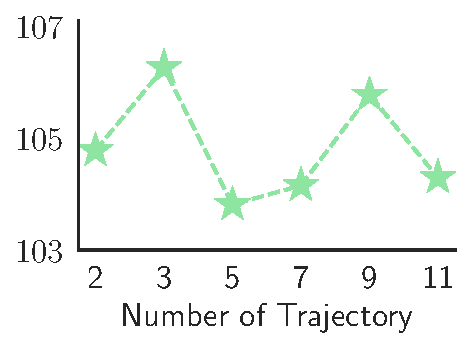
\includegraphics[width=\textwidth]{./Tex/fig/ListNet_p=1_line.pdf}
         \captionsetup{font=small}
         \vspace{-6mm}
         \caption{\rewardnet}
         \label{fig:listnet_p1_num_traj}
     \end{subfigure}
     \hfill
     \begin{subfigure}[b]{0.24\textwidth}
         \centering
         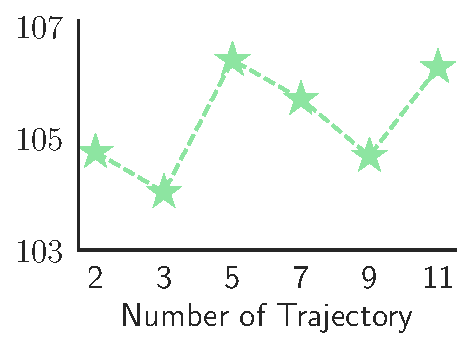
\includegraphics[width=\textwidth]{./Tex/fig/listMLE_softmax_line.pdf}
         \captionsetup{font=small}
         \vspace{-6mm}
         \caption{\rewardmle}
         \label{fig:listmle_smax_num_traj}
     \end{subfigure}
     \hfill
    %  \rulesep
    \begin{subfigure}[b]{0.24\textwidth}
         \centering
         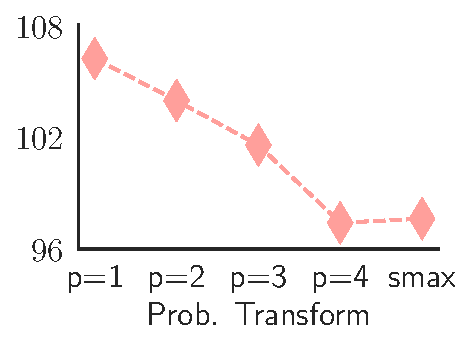
\includegraphics[width=\textwidth]{./Tex/fig/listNet_3_line.pdf}
         \captionsetup{font=small}
         \vspace{-6mm}
         \caption{\rewardnet}
         \label{fig:listnet_3_transf}
     \end{subfigure}
     \hfill
     \begin{subfigure}[b]{0.24\textwidth}
         \centering
         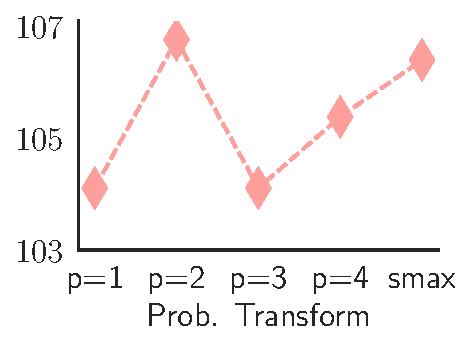
\includegraphics[width=\textwidth]{./Tex/fig/ListMLE_5_line.pdf}
         \captionsetup{font=small}
         \vspace{-6mm}
         \caption{\rewardmle}
         \label{fig:listmle_5_transf}
     \end{subfigure}
     \vspace{-2mm}
     \captionsetup{font=small}
        \caption{ 
        \footnotesize{Line plots comparing the Combined Score when the \rewardnet and \rewardmle losses are constructed under a different number of sampled trajectories or different probabilistic transforms.
        The $y$-axis represents the Combined Score.
        $p=1,2,3,4$ is the escort transform with power $1,2,3,4$.
        ``smax" is the softmax transform.
        Results are the average over five random seeds.}
        }
        \label{fig:abla_sweep}
        \vspace{-1.5em}
\end{figure}

\textbf{(b):}~\textit{Do different probabilistic transforms in reward learning objectives affect the performance?}
We modify the basic version of the \rewardnet and \rewardmle models in Table~\ref{table:main} by using the softmax transform and by using different powers in the escort transform in the reward learning losses Eqs.~\eqref{eq:listnet} and \eqref{eq:listmle}.
For the escort transform, we consider $\Phi=(\cdot)^p, p\in \cbr{1,2,3,4}$.

Figs.~\ref{fig:listnet_3_transf} and \ref{fig:listmle_5_transf} plot the resulting Combined Scores.
We see that the \rewardmle model is less sensitive to the choice of probabilistic transform --- all the considered variants have a Combined Score of at least $104$.
In fact, changing its softmax transform used in Table~\ref{table:main} to the escort transform with power two improves the performance to $106.77$.
Thus, the choice of probabilistic transform provides an additional angle to improve the learned reward function and the entire ToD model.

\begin{figure}[tb]
     \vspace{-2mm}
     \centering
     \begin{subfigure}[b]{0.24\textwidth}
         \centering
         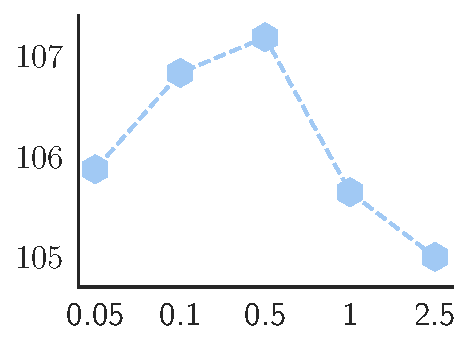
\includegraphics[width=\textwidth]{./Tex/fig/comb_alpha_line.pdf}
         \captionsetup{font=small}
         \vspace{-6mm}
         \caption{\footnotesize{Combined Score}}
         \label{fig:vary_alpha_comb}
     \end{subfigure}
     \hfill
     \begin{subfigure}[b]{0.24\textwidth}
         \centering
         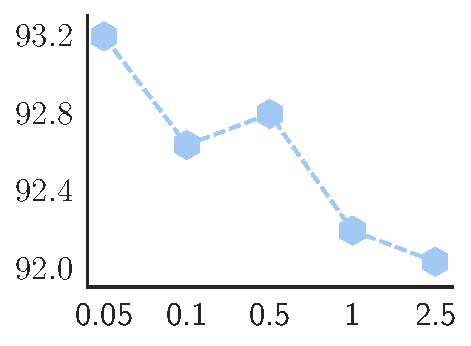
\includegraphics[width=\textwidth]{./Tex/fig/inform_alpha_line.pdf}
         \captionsetup{font=small}
         \vspace{-6mm}
         \caption{\footnotesize{Inform Rate}}
         \label{fig:vary_alpha_inform}
     \end{subfigure}
     \hfill
    %  \rulesep
    \begin{subfigure}[b]{0.24\textwidth}
         \centering
         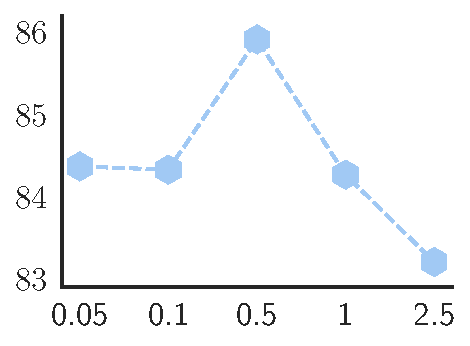
\includegraphics[width=\textwidth]{./Tex/fig/success_alpha_line.pdf}
         \captionsetup{font=small}
         \vspace{-6mm}
         \caption{\footnotesize{Success Rate}}
         \label{fig:vary_alpha_success}
     \end{subfigure}
     \hfill
     \begin{subfigure}[b]{0.24\textwidth}
         \centering
         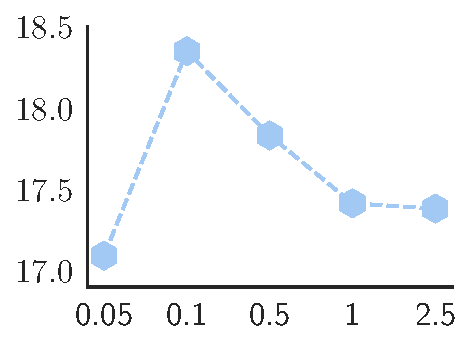
\includegraphics[width=\textwidth]{./Tex/fig/bleu_alpha_line.pdf}
         \captionsetup{font=small}
         \vspace{-6mm}
         \caption{\footnotesize{BLEU Score}}
         \label{fig:vary_alpha_bleu}
     \end{subfigure}
     \vspace{-3mm}
     \captionsetup{font=small}
        \caption{ 
        Line plots showing the four automatic evaluation metrics of the \rewardnet + GS model in Table~\ref{table:main} under different $\alpha$ values in the generation-model loss Eq.~\eqref{eq:loss_gen}.
        Results are the average over five seeds.
        }
        \label{fig:vary_alpha}
        \vspace{-5mm}
\end{figure}

\textbf{(c):}~\textit{Is our method sensitive to the coefficient $\alpha$ in the generation-model loss Eq.~\eqref{eq:loss_gen}?}
To investigate the robustness of our method under different weights for the policy-gradient optimization of the response-generation model.
We select our best policy-gradient-based model in Table~\ref{table:main}, the \rewardnet + GS model, and vary the $\alpha$ coefficient in the generation-model loss Eq.~\eqref{eq:loss_gen}.
Fig.~\ref{fig:vary_alpha} plots the resulting four automatic evaluation metrics.

We see that our model is relatively robust to the choice of $\alpha$.
The five variants in Fig.~\ref{fig:vary_alpha} all have Combined Scores of at least $105$, higher than the best baseline result of $104.78$ in Table~\ref{table:main}.
In fact, by changing the $\alpha$ coefficient  to $0.5$ from $0.1$ used in Table~\ref{table:main}, we achieve a \emph{even better} Combined Score of $\approx 107.2$.
Further, the capability of task completion and the fluency of the generated responses are both relatively insensitive to the choice of $\alpha$.

\textbf{(d):}~\textit{How does the addition of the policy-gradient method Gumbel-softmax help the performance?}
Fig.~\ref{fig:abla_gs} compares the performance of our models in Table~\ref{table:main}, with error bars showing the standard deviation of the Combined Score over five seeds.
It is clear that the addition of the Gumbel-softmax method can not only improve the score but also reduce the performance variation, which is apparent when comparing the \rewardmle model with the \rewardmle + GS model.

As discussed in \Secref{sec:main_gs}, the Gumbel-softmax (GS) trick can be more advantageous than the classical REINFORCE method \citep{reinforce1992} for the policy-gradient update.
As a demonstration, we conduct a toy experiment following \citet{arsm2019} and plot the results in Fig.~\ref{fig:abla_toy}.
The task here is to learn the parameter $\vpsi$ of a $D$-dimensional categorical distribution to maximize a simple reward function.
Specifically, denote the sigmoid function as $\sigma(\cdot)$, the goal is
\begin{equation*}\textstyle
    \max_{\vpsi \in \R^D} \E_{x \sim \mathrm{Cate}(\sigma(\vpsi))}\sbr{f(x)},\quad f(x) \triangleq 0.5 + x / (D \cdot R),\; \forall\, x \in \cbr{1, \ldots, D}, 
\end{equation*}
where $\mathrm{Cate}(\sigma(\vpsi))$ denotes the categorical distribution with probability vector $\sigma(\vpsi)$, and $D=R=30$.
The best $\sigma(\vpsi)$ is $(0,\ldots,0,1)$, leading to the optimal expected reward of $\approx 0.533$.
We initialize $\vpsi = \vzero$ and use one sample for the stochastic gradient-ascent update, with a learning rate of $1.0$.

The first row of Fig.~\ref{fig:abla_toy} traces the objective function during the training process when using the true gradient, REINFORCE, and the GS for policy-gradient updates.
We see that the REINFORCE method converges to a local maximum, while the GS method reaches the global optimum, as using the true gradient for updates.
The second row shows the gradients for $\theta_1$ and $\theta_D$, where we see that gradient estimates from the REINFORCE method are both unstable and vanishing, compared to the GS method.
The learned probabilities $\cbr{\sigma(\vpsi)_1, \ldots, \sigma(\vpsi)_D}$ is traced in the third row, where the red line is for $\sigma(\vpsi)_D$ that should ideally be $1$, and the shadowed lines are for the other components that ought to be $0$.
The learning process of the GS method closely resembles that of using the true gradient, while REINFORCE oscillates around a local optimum.
The last row of Fig.~\ref{fig:abla_toy} plots the estimate of gradient variance via $500$ samples, averaged over each component of the $\vpsi$ vector.
The gradient variance of the REINFORCE method is on the order of $10^{-2}$ at the beginning and converges to roughly $10^{-4}$, while the GS is $10^{-6}$ throughout the training process.
This toy experiment shows that a low-variance method, such as the GS, can be critical to the success of policy-gradient training.




\begin{figure}[tb]
\vspace{-2mm}
    \centering
    \begin{minipage}{0.49\textwidth}
        \centering
        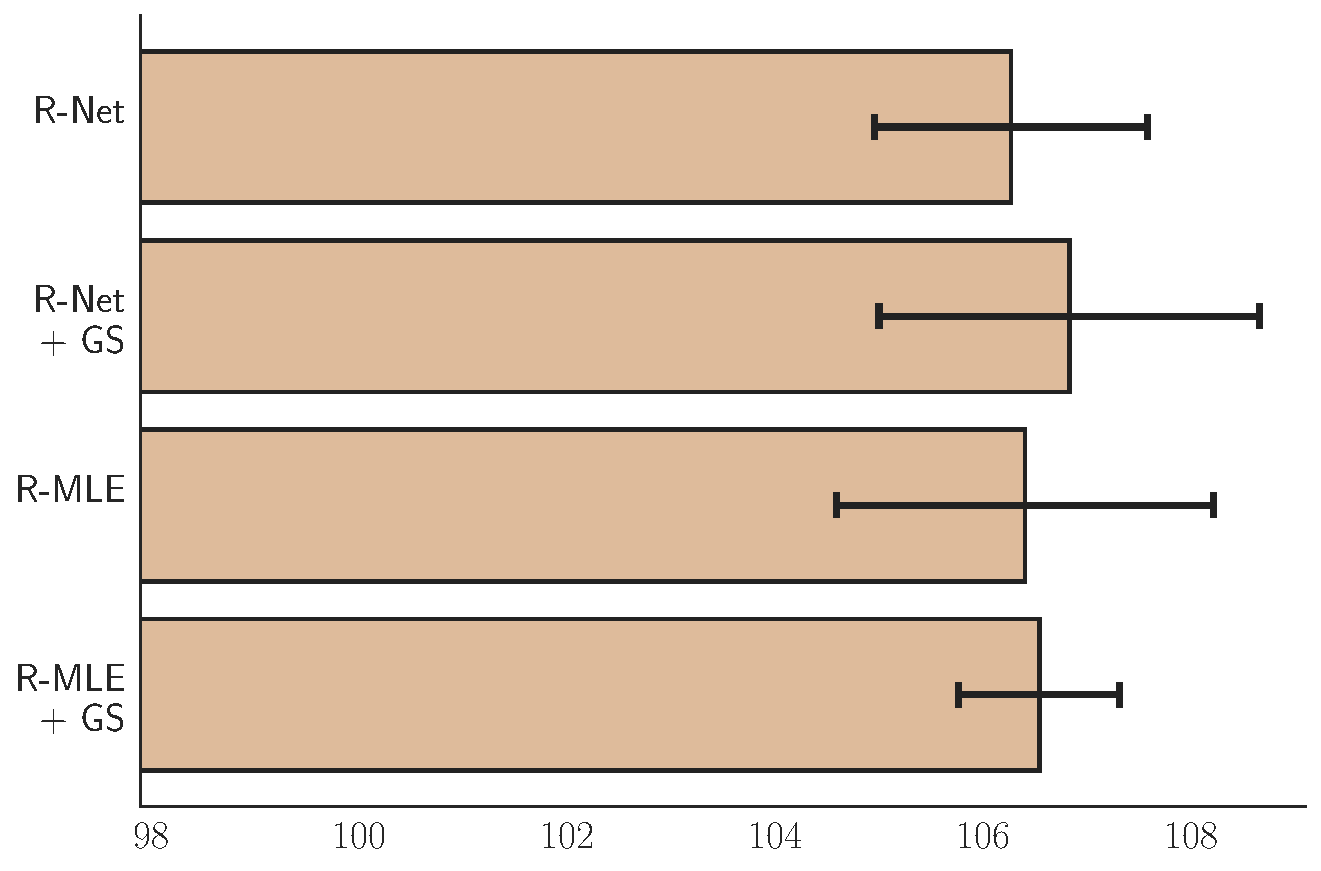
\includegraphics[width=1\linewidth]{./Tex/fig/w_wo_gs_bar.pdf}
        \captionsetup{font=small}
        \vspace{-2em}
        \caption{\footnotesize{ Bar plot comparing our four models in Table~\ref{table:main}.
        Mean and one standard deviation over five random seeds are shown.
        ``R-Net" denotes \rewardnet. ``R-MLE" is \rewardmle. ``GS" is Gumbel-softmax.
        }}
        \label{fig:abla_gs}
    \end{minipage}
    \hfill
    \begin{minipage}{0.49\textwidth}
        \centering
        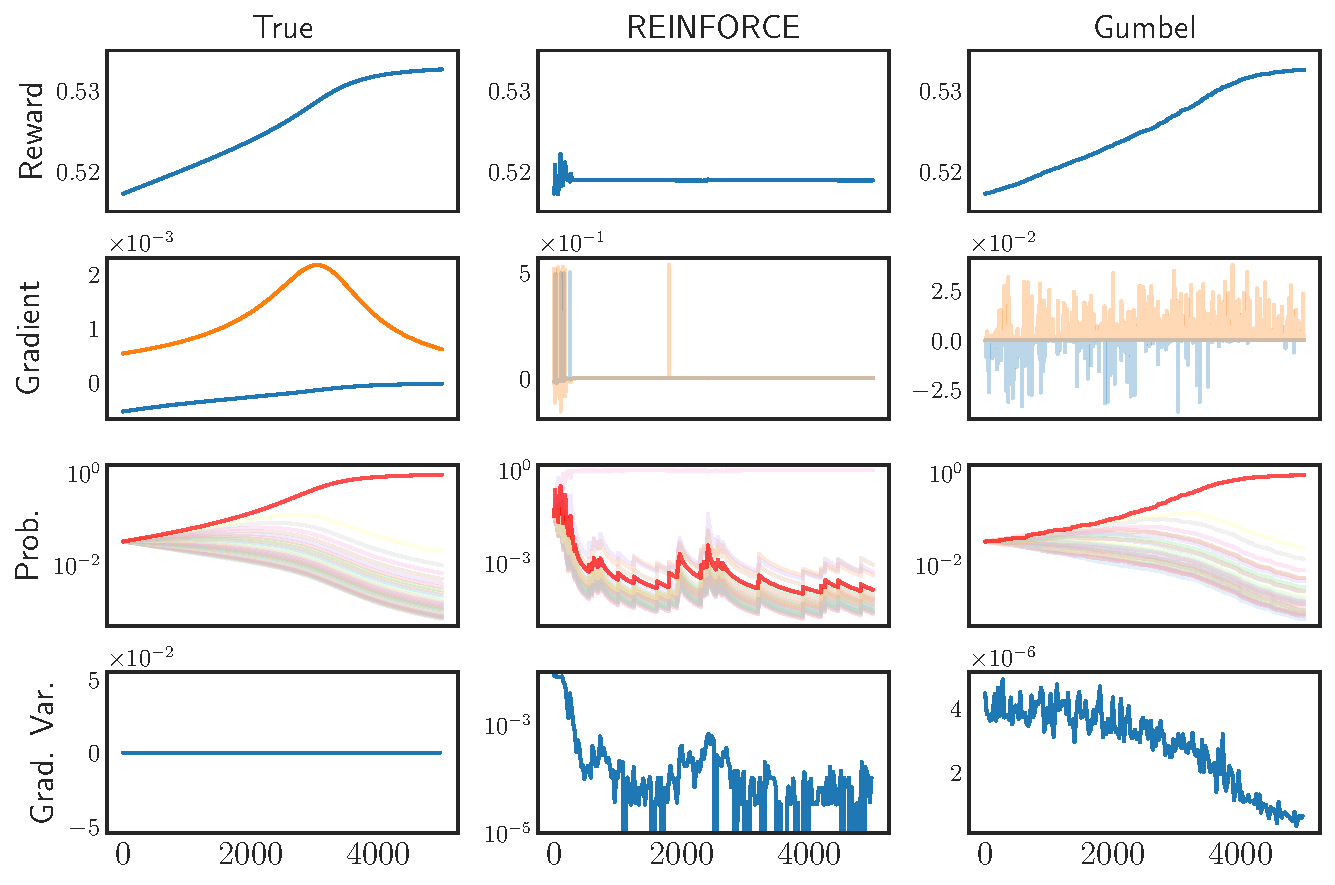
\includegraphics[width=1\linewidth]{./Tex/fig/gs_gradient_var_plot.pdf} % figsize=(9, 6)
        \captionsetup{font=small}
        \vspace{-2em}
        \caption{\footnotesize{Toy experiment comparing REINFORCE and Gumbel-softmax in reward maximization, the estimated gradients, the estimated probabilities, and the gradient variance.
        See \Secref{sec:exp_abla} for details.}}
        \label{fig:abla_toy}
    \end{minipage}
    \vspace{-.8em}
\end{figure}




\begin{figure}[tb]
    \centering
    \begin{minipage}{0.49\textwidth}
        \centering
     \begin{subfigure}[b]{0.48\textwidth}
         \centering
         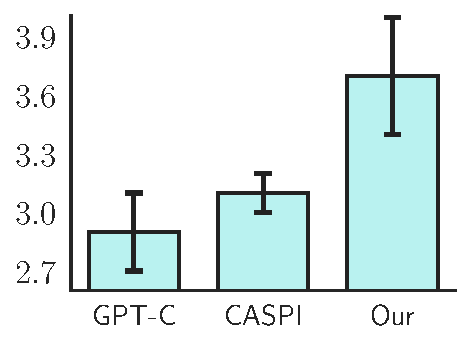
\includegraphics[width=\textwidth]{./Tex/fig/appropriate_bar.pdf}
         \captionsetup{font=small}
         \vspace{-6mm}
         \caption{Appropriateness}
         \label{fig:appropriate}
     \end{subfigure}
     \hfill
     \begin{subfigure}[b]{0.48\textwidth}
         \centering
         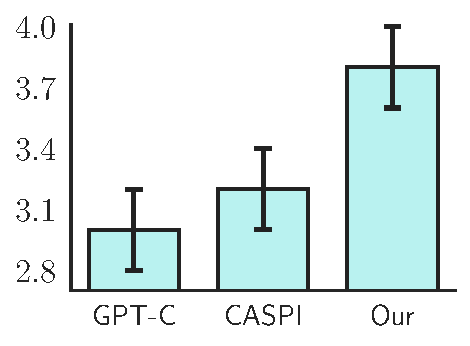
\includegraphics[width=\textwidth]{./Tex/fig/fluency_bar.pdf}
         \captionsetup{font=small}
         \vspace{-6mm}
         \caption{Fluency}
         \label{fig:fluency}
     \end{subfigure}
     \vspace{-3mm}
     \captionsetup{font=small}
        \caption{ 
        \footnotesize{Bar plots for the results of human evaluation on appropriateness and fluency, showing the mean and one standard deviation of each method. 
        The scores are on a $5$ scale and higher scores indicate better results.
        ``GPT-C" denotes GPT-Critic.
        Details for the setup of human evaluation are discussed in \Secref{sec:exp_further}.}
        }
        \label{fig:human_eval}
    \end{minipage}
    \hfill
    \begin{minipage}{0.49\textwidth}
        \centering
     \begin{subfigure}[b]{0.48\textwidth}
         \centering
         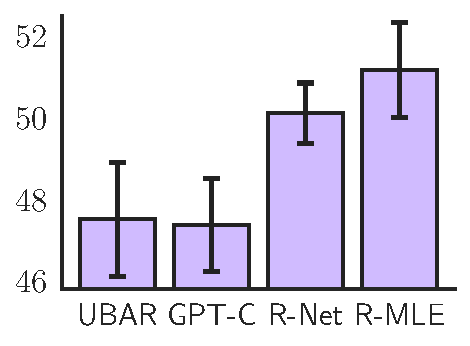
\includegraphics[width=\textwidth]{./Tex/fig/joint_acc_bar.pdf}
         \captionsetup{font=small}
         \vspace{-6mm}
         \caption{Joint Accuracy}
         \label{fig:dst_joint_acc}
     \end{subfigure}
     \hfill
     \begin{subfigure}[b]{0.48\textwidth}
         \centering
         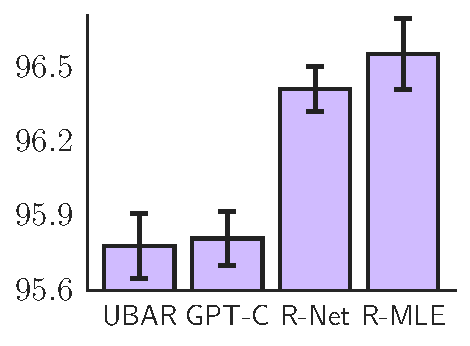
\includegraphics[width=\textwidth]{./Tex/fig/slot_acc_bar.pdf}
         \captionsetup{font=small}
         \vspace{-6mm}
         \caption{Slot Accuracy}
         \label{fig:dst_slot_acc}
     \end{subfigure}
     \vspace{-3mm}
     \captionsetup{font=small}
        \caption{ 
       \footnotesize{ Bar plots for the quality of the generated dialogue states, showing the mean and standard deviation of two metrics.
        ``GPT-C" denotes GPT-Critic, ``R-Net" denotes \rewardnet, ``R-MLE" is \rewardmle.
        The results of UBAR and GPT-Critic are from \citet{gptcritic2022}.
        Our results are over five random seeds.}
        }
        \label{fig:further_dst}
    \end{minipage}
    \vspace{-1.2em}
\end{figure}




\vspace{-.5em}
\subsection{Further Analysis} \label{sec:exp_further}
\vspace{-.5em}

\myparagraph{Human evaluation.}
For a more comprehensive evaluation of our method, we conduct a human evaluation on the quality of the generated responses, where our model and the top two baselines in Table~\ref{table:main}, GPT-Critic and CASPI, are compared.
We follow the evaluation protocol in prior work \citep[\eg,][]{damd2020,caspi2021,gptcritic2022} to evaluate on two metrics:
1) \textbf{Appropriateness}: measures the appropriateness of the generated response under the context of the dialogue turn;
2) \textbf{Fluency}: evaluates the comprehensibility and coherency of the generated response.
We randomly picked $50$ turns in the test set and showed to $10$ evaluators the responses generated from each method, together with the dialogue history up to that turn.  
The method names were anonymized.
The evaluators were asked to read the dialogue history and score the response on a $5$-Point Likert Scale $\cbr{1,2,3,4,5}$, where score $5$ is the highest and $1$ the lowest.

Fig.~\ref{fig:human_eval} summarizes the evaluation results.
We see that our model outperforms the baselines in both the appropriateness and fluency scores.
The human-evaluation results coincide with our comparatively good dialogue-task completion and BLEU score in
Table~\ref{table:main}.

\myparagraph{Examples of the generated dialogues.}
Tables~\ref{table:dia_pmul4610} and \ref{table:dia_sng1012} in Appendix~\ref{sec:appendix_example} conduct two case studies comparing the generated responses from our method with those from the baselines GPT-Critic and CASPI.
We additionally annotate the generated responses to discuss the quality of those generations.
These examples show that the responses from our model compare favorably with the baselines in both task completion and comprehensibility, aligning with the automatic and human evaluations.

\myparagraph{Quality of the DST.}
To further understand the performance gain of our models, we compare our basic \rewardnet and \rewardmle models in Table~\ref{table:main} with the baselines UBAR and GPT-Critic on the quality of the generated dialogue states.
Fig.~\ref{fig:further_dst} plots the results of the dialogue state prediction, measured by the two metrics Joint (Goal) Accuracy and Slot Accuracy \citep{wu2019transferable}.
We see that our two models have more accurate DST than the two baselines, which can be related to their better performance in Table~\ref{table:main}.
Interestingly, the DST of the \rewardmle model is also better than that of the \rewardnet model. 
This may suggest that a better reward model not only benefits the learning of response generation, but also the DST. 
These two losses are jointly minimized in training the ToD model, and thus a good response-generation loss from a better reward model may help the optimization of the DST loss.


